\subsection{Aliasing}
    \begin{align*}
        y_1[k] &= cos(\omega k T_s), &&k = 0, 1, 2\\
        y_2[k] &= cos((\omega + n\frac{2\pi}{T_s})k T_s), &&n = 0, 1, 2\\
        &= cos(\omega k T_s + \text{\cancel{$n2\pi k$}}) = y_1[k]
    \end{align*}
    \centerline{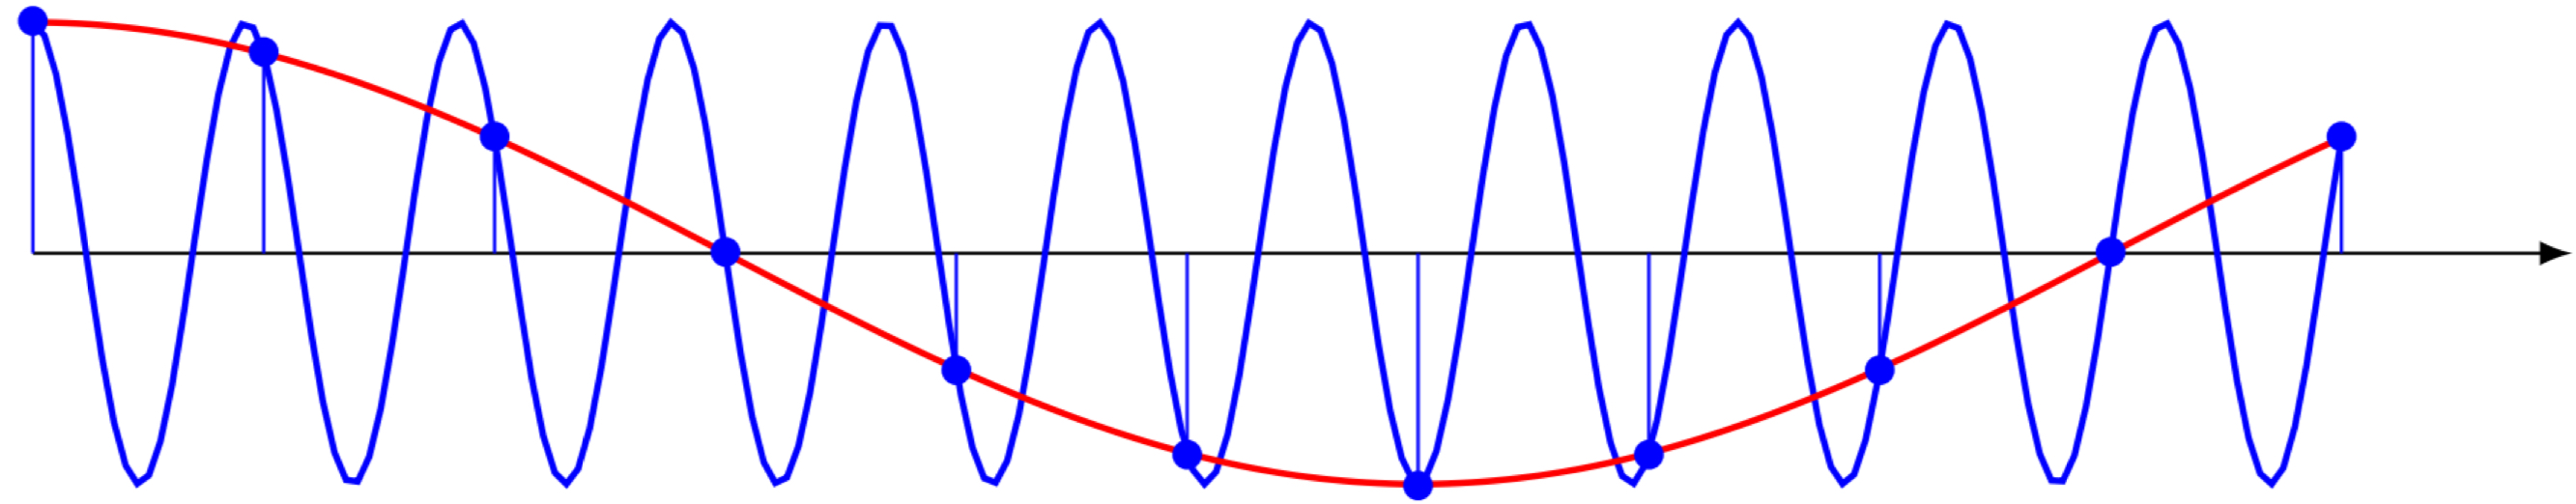
\includegraphics[width=0.8\linewidth]{src/1_discrete_time/images/aliasing.jpg}}
    \vspace{0pt}

    \subsubsection{Nyquist-Shannon Sampling theorem}
        $$
        f_N = \frac{1}{2T_s}\left[\text{Hz}\right] \quad \text{or} \quad \omega_N = \frac{\pi}{T_s}\left[\frac{\text{rad}}{\text{s}}\right]
        $$

        \centerline{\textbf{No aliasing if $\omega < \omega_N$!}}